\documentclass{beamer}
\usetheme[
  block=fill,
  background=dark,
  titleformat=smallcaps,
  progressbar=frametitle,
  numbering=none,
]{metropolis}

% Math
\usepackage{amsmath}
\usepackage{amssymb}
\usepackage{stmaryrd}

% Code listing
\usepackage{minted}
\usemintedstyle{monokai}
%\usemintedstyle{native}
%\usemintedstyle{tango}
\newcommand{\icode}[1]{\mintinline{haskell}{#1}}

% Graphics
\usepackage{graphics}
\usepackage{pdfpages}
\graphicspath{{figures/}} % Location of the graphics files

\newcommand\todo[1]{\textcolor{red}{#1}}

% Box macro
\newcommand{\ex}[2]{
  \vfill
  \begin{alertblock}{#1}
    #2
  \end{alertblock}
}
%----------------------------------------------------------------------------

% Beamer
\title{AlgoRhythm}
\subtitle{A Library for Algorithmic Music Composition}
\author{Joris ten Tusscher, Cas van der Rest, Orestis Melkonian}
\date{April 5, 2018}
\institute{Universiteit Utrecht}

\begin{document}
	\maketitle
	
	\begin{frame}{Music DSL}
	\todo{music representation (Music, MusicCore, Scale, Chord, etc...}\\
	\todo{music manipulation (transpose, retrograde, time-scale, etc...}\\
	\end{frame}
		
	{\usebackgroundtemplate{%
  	
\includegraphics[width=\paperwidth,height=\paperheight]{no-analysis.png}}
	\begin{frame}{Focus on Generation, Ignore Analysis}
	\end{frame}
	}	
	
	\begin{frame}{Generation}
	\todo{genState, selectors, diatonic improv, etc...}
	\end{frame}
	
	\begin{frame}{Dynamic Performance}
	\todo{k-means, etc...}
	\end{frame}
	
	\begin{frame}{Grammars}
	\todo{grammar description}\\
	\end{frame}
	
	\begin{frame}[fragile=singleslide]{Grammars: Tabla Rhythm}
	\begin{minted}[baselinestretch=1, fontsize=\small, autogobble]{haskell}
tabla :: Grammar () Syllable
tabla = S |:
  [ S |--> TE1 :-: XI
  , XI |--> TA7 :-: XD
  , XD |--> TA8
  , XG |--> TB2 :-: XA
  ...
  , TE4 |--> Ti :-: Rest :-: Dha :-: Ti
  , TC2 |--> Tr :-: Kt
  , TB3 |--> Dha :-: Tr :-: Kt
  , TD1 |--> Rest
  ...
  ]
instance ToMusicCore Syllable where
    ...
	\end{minted}
	\end{frame}
	
	\begin{frame}[fragile=singleslide]{Grammars: Jazz Improvisation}
	\begin{minted}[baselinestretch=0.8, fontsize=\footnotesize, autogobble]{haskell}
melody :: Grammar () NT
melody = MQ |:
  [ -- Abstract Rhythm { MQ ~> Q }
    (MQ, 1, (== qn))     |-> Q%:qn
  , (MQ, 25, (> (hn^.)))  :-> \t -> Q%:hn :-: MQ%:(t - hn)
  ...
    -- Concrete Rhythm { Q ~> MN }
  , (Q, 47, (== wn)) |-> MN%:qn :-: Q%:hn :-: MN%:qn
  , (Q,  6, (== hn)) |-> HT%:(qn^^^) :-: HT%:(qn^^^) :-: HT%:(qn^^^)
  ...
  -- Abstract Melody { MN ~> N }
  , (MN, 1, (== wn)) |-> MN%:qn :-: MN%:qn :-: MN%:qn :-: MN%:qn
  , (MN,  1, (== qn)) |-> HT%:(en^^^) :-: HT%:(en^^^) :-: AT%:(en^^^)
    ...
  -- Concrete Melody { N ~> NT }
  , (N, 50, (== qn)) |-> ColorTone%:qn
  , (N, 45, (== qn)) |-> Rest%:qn
  , (N,  1, (== en)) |-> ApproachTone%:en
  ...
  ]

mkSolo :: Music SemiChord -> Music NT -> IO Melody
    \end{minted}
	\end{frame}

	\begin{frame}[fragile=singleslide]{Grammars: Tonal Harmony}
	\begin{minted}[baselinestretch=0.8, fontsize=\footnotesize, autogobble]{haskell}
harmony :: Grammar Modulation Degree
harmony = I |:
  [ -- Turn-arounds
    (I, 8, (> wn)) :->
      \t -> Let (I%:t/2) (\x -> x :-: x)
  , (I, 6, (> hn) /\ (<= wn)) :->
      \t -> II%:t/4 :-: V%:t/4 :-: I%:t/2
  , (I, 2, (> hn) /\ (<= wn)) :->
      \t -> V%:t/2 :-: I%:t/2
  , (I, 2) -|| (<= wn)
    -- Modulations
  , (V, 5, (> hn)) :-> \t -> Modulation P5 $: I%:t
  , V -| 3
  , (II, 2, (> hn)) :-> \t -> Modulation M2 |$: I%:t
  , II -| 8
  ]

instance Expand Degree Modulation SemiChord where
    ...

voiceLead :: Music SemiChord -> IO (Music Chord)
	\end{minted}
	\end{frame}
	
	\begin{frame}[fragile=singleslide]{Demo: Code}
	\begin{minted}[baselinestretch=0.9, fontsize=\footnotesize, autogobble]{haskell}
    orientalAlgebras = do
      let ?harmonyConfig = HarmonyConfig
        { basePc  = A
        , baseOct = Oct3
        , baseScale = arabian
        , chords  = equally allChords
        }
      let ?melodyConfig = defMelodyConfig
        { scales  = equally allScales
        , octaves = [(20, Oct4), (15, Oct5), (5, Oct6)]
        , colorWeight = 0
        , approachWeight = 10
        }
      let ?midiConfig = MIDIConfig (6%5) [Piano, Sitar, Tabla]
      let ?tablaBeat = sn
      
      (back, fore) <- integrate (12 * wn)
      rhythm <- runGrammar tabla (12 * wn) ()
      writeToMidiFile "out.mid" (dyn (back :=: fore :=: rhythm))
	\end{minted}
  	\end{frame}
	
	\begin{frame}{Demo: Music score}
	\vspace{-.5cm}
	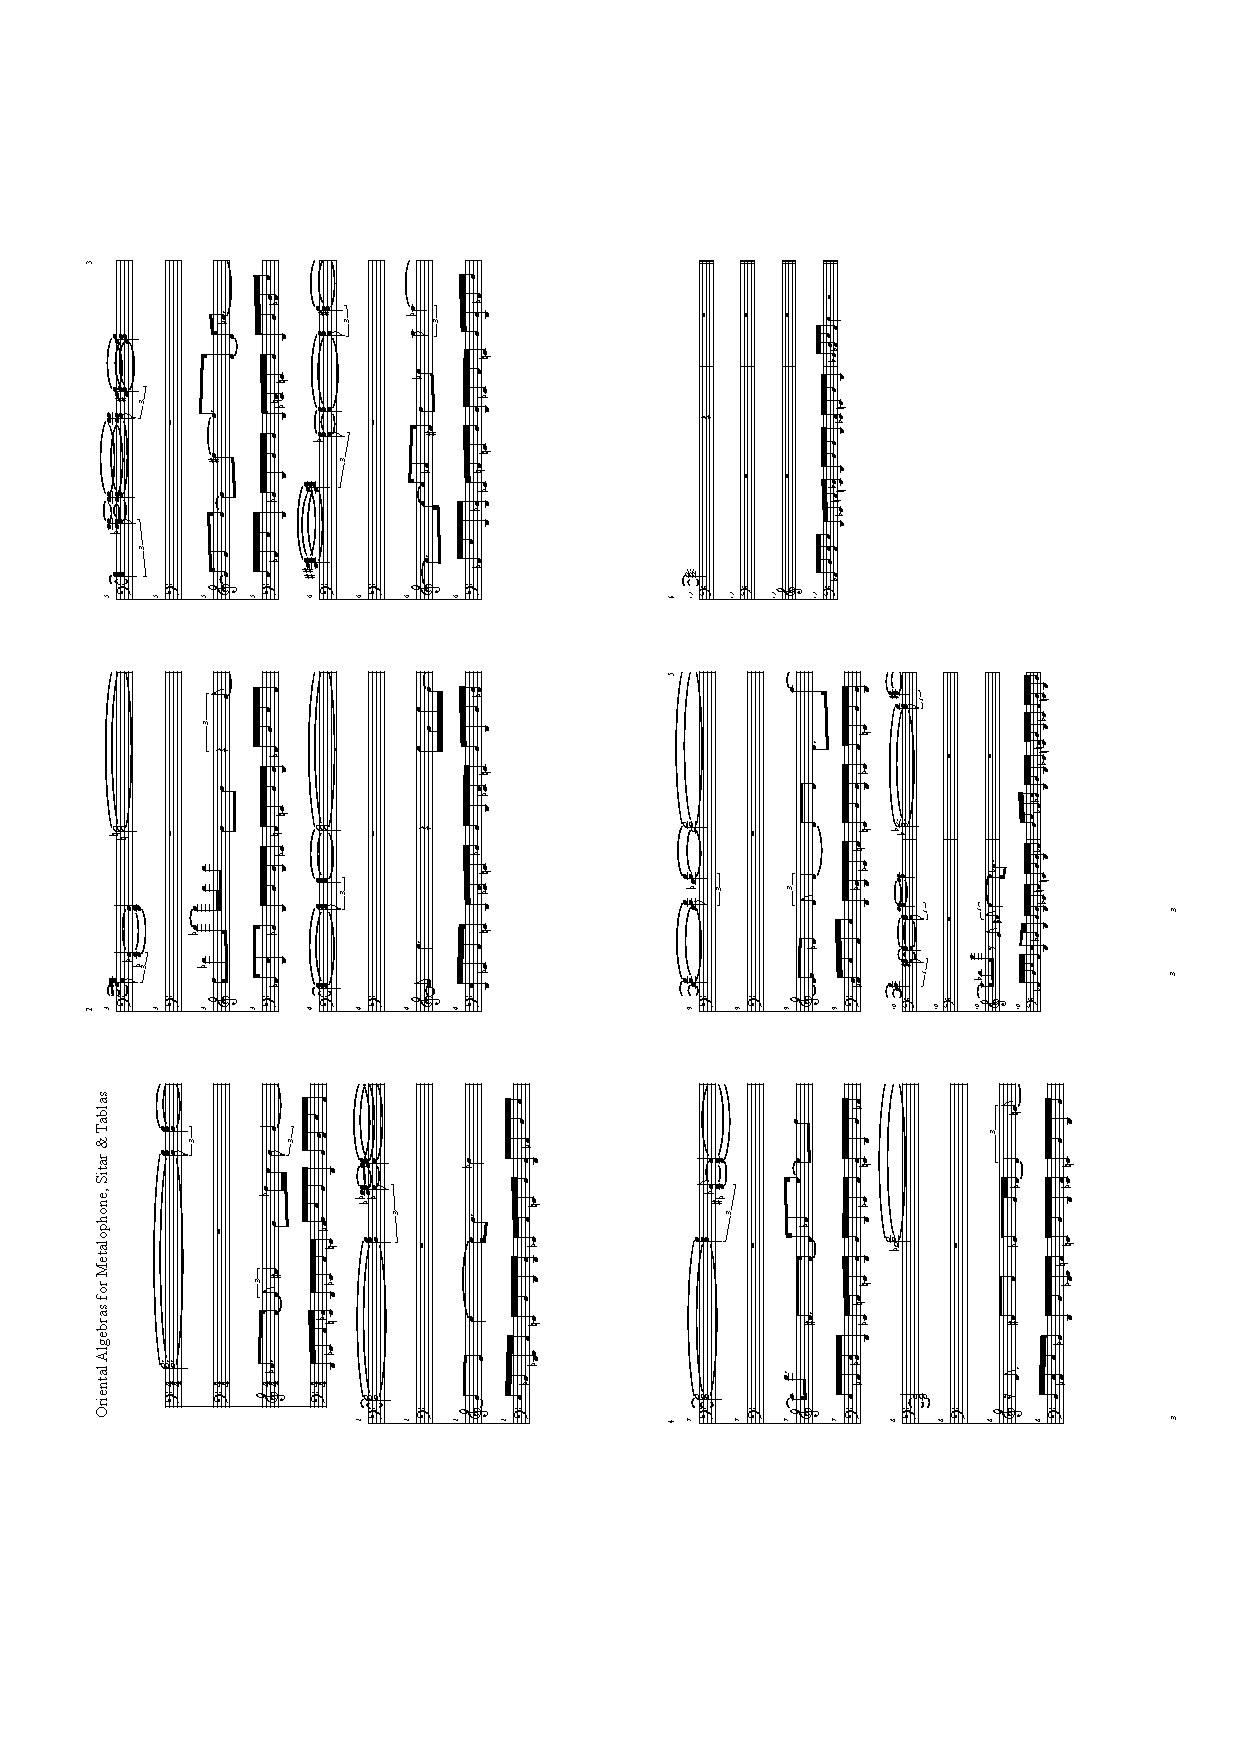
\includegraphics[scale=.42,angle=-90]{oriental.pdf}
	\end{frame}
  	
\end{document}
